%-----------------------------------------------------------------------------
%
%               Template for sigplanconf LaTeX Class
%
% Name:         sigplanconf-template.tex
%
% Purpose:      A template for sigplanconf.cls, which is a LaTeX 2e class
%               file for SIGPLAN conference proceedings.
%
% Guide:        Refer to "Author's Guide to the ACM SIGPLAN Class,"
%               sigplanconf-guide.pdf
%
% Author:       Paul C. Anagnostopoulos
%               Windfall Software
%               978 371-2316
%               paul@windfall.com
%
% Created:      15 February 2005
%
%-----------------------------------------------------------------------------


%\documentclass[10pt,preprint,reprint]{sigplanconf}
\documentclass[10pt,reprint]{sigplanconf}

% The following \documentclass options may be useful:

% preprint      Remove this option only once the paper is in final form.
% 10pt          To set in 10-point type instead of 9-point.
% 11pt          To set in 11-point type instead of 9-point.
% authoryear    To obtain author/year citation style instead of numeric.

\usepackage{amsmath}


\begin{document}

\special{papersize=8.5in,11in}
\setlength{\pdfpageheight}{\paperheight}
\setlength{\pdfpagewidth}{\paperwidth}

\conferenceinfo{CONF 'yy}{Month d--d, 20yy, City, ST, Country} 
\copyrightyear{20yy} 
\copyrightdata{978-1-nnnn-nnnn-n/yy/mm} 
\doi{nnnnnnn.nnnnnnn}

% Uncomment one of the following two, if you are not going for the 
% traditional copyright transfer agreement.

%\exclusivelicense                % ACM gets exclusive license to publish, 
                                  % you retain copyright

\permissiontopublish             % ACM gets nonexclusive license to publish
                                  % (paid open-access papers, 
                                  % short abstracts)

\titlebanner{banner above paper title}        % These are ignored unless
\preprintfooter{short description of paper}   % 'preprint' option specified.

\title{WebCUDA: Enabling High Performance Something}
%\subtitle{Subtitle Text, if any}

\authorinfo{Jiho Choi}
           {University of Illinois in Urbana-Champaign}
           {jchoi42@illinois.edu}
\authorinfo{Kurt Fellows}
           {University of Illinois in Urbana-Champaign}
           {fellows2@illinois.edu}
\authorinfo{Tom Shull}
           {University of Illinois in Urbana-Champaign}
           {shull1@illinois.edu}

\maketitle

\begin{abstract}
	
This document provides instructions for submitting papers to the 19th
International Conference on Architectural Support for Programming Languages
and Operating Systems (ASPLOS), 2014.  It also provides a sample for how
papers must be formatted.


\end{abstract}

\category{CR-number}{subcategory}{third-level}

% general terms are not compulsory anymore, 
% you may leave them out
\terms
term1, term2

\keywords
keyword1, keyword2

\section{Introduction}
\label{intro}
(
JavaScript is one of the top 10 most popular programming languages, 
considered by many as the “assembly language of the Internet.” JavaScript is
prevalent in the vast majority of websites due to it being the only
ubiquitous, cross-platform scripting language available on the browser. The 
burgeoning mobile device market has also increased the importance of JavaScript due
to their contribution to the growing  popularity of web applications.
%The growing
%mobile device market will continue to boost the popularity of web applications.
Due to the importance of JavaScript, major web browser providers competitively
enhance their JavaScript engines. These improvements in JavaScript performance
have allowed for a proliferation in both the number of web applications and
their capabilities.  

However, currently JavaScript's single-threaded execution model fundamentally limits
performance and hinders adoption for computationally intensive and rich visual
computing applications on the web, such as 3D games, video processing
applications, and augmented reality applications. Such applications have much data
parallelism and can benefit from processing elements available in today’s
heterogeneous systems, such as Graphic Processing Units (GPUs).  Furthermore,
JavaScript is gaining attention on the server-side as well through popular
projects such as NodeJS \cite{nodeJS}, where operations are often
computationally intensive or data-parallel, expanding the JavaScript application
domain which can benefit from heterogeneous systems.

We propose a JavaScript language extension for CUDA bindings, providing portable
and efficient access to CUDA-enabled GPUs from web applications.  We call this
project \namens, highlighting the enabling of CUDA programming from within the
browser domain. Our contributions in this paper are as follows:

%In addition to evaluating the performance impact using the real hardware, we
%plan to integrate the JavaScript engine with a heterogeneous system simulator to
%experiment with various architectural alternatives starting with the memory
%model of GPUs. We envision this to be the first steps towards a long-term goal
%of creating heterogeneous systems specialized for JavaScript execution.  

\begin{itemize}

\item Define JavaScript extension to allow CUDA bindings within JavaScript code
\item Implement \name specification within a state of the art JavaScript compiler
\item Compare the performance of native CUDA, CUDA-enabled JavaScript, and native JavaScript benchmarks
\item Analyze overheads of the \name runtime.
\item Provide insights on the flexibility of adding extensions into V8

\end{itemize}

Our evaluations show that \name is able to achieve a speedup of XX\% over
JavaScript Applications without impacting native JavaScript performance.
Providing web developers access to high-performance, parallel computational
resources will not only enable more existing applications to be ported to the
web environment, but will also unleash a wave of creativity resulting in new
innovative web applications.

This paper is organized as follows: Section~\ref{background} provides background
about JavaScript and CUDA, Sections \ref{overview} and \ref{imp} describe the
structure and implementation of \namens, and Section~\ref{eval} demonstrates the
performance benefits of \namens. Finally, Section~\ref{disc} provides discussion
about our project, Section~\ref{related} highlights related work, and
Section~\ref{conc} concludes.



\section{Background}
\label{background}

This section provides readers background about the JavaScript and CUDA
programming environments. Experienced programmers in these domains can skip to
Sections~\ref{overview} and \ref{imp} to learn about our specification and
implementation of \namens.

\subsection{JavaScript} JavaScript, also known as ECMAScript, is a
dynamically-typed, object-oriented scripting language.  It has gained popularity
through its use in the web domain. JavaScript is the de facto standard for
adding animations to web pages. Programmers are able to create JavaScript events
that are triggered by specific user interaction with the web page. These
JavaScript events can manipulate the web page layout through altering the web
page's Document Object Model (DOM), an abstraction of the web page provided by
browsers. By using JSON~\cite{json}, JavaScript programs can also asynchronously
communicate with servers and update content on a web page without having to
reload. In addition, there is a large collection of libraries, such as
JQuery~\cite{JQuery}, used by programmers to provide users interactive browsing
experiences.

JavaScript is run either by an interpreter or Just-In-Time Compilation. In the
JavaScript world, all variables are objects and thus can have fields and methods
added to and removed from them on the fly. This limits the amount of
optimization able to be performed, since the fields and objects are not static. In
addition, JavaScript has a single-threaded execution model, which further limits
its performance.

\subsection{CUDA} Graphics processing units (GPUs), as their name suggests, were
initially designed to accelerate computationally intensive graphics rendering.
However, in the past decade or so, a large push has been made to make the
processing resources available on GPUs more accessible for general purpose use.
CUDA is a parallel programming platform developed by NVIDIA which allows
programmers access to the graphics processing units. CUDA provides extensions to
standard programming languages like C/C++ and Fortran to give programmers in
these languages the option to move computation from more latency oriented CPUs
to bandwidth oriented GPUs. The Khronos group has standardized OpenCL
\cite{openCL}, a programming platform similar to CUDA which allows programs to
execute across heterogeneous systems.  

CUDA code is often divided into two parts: one part is the code designed to
execute on the CPU or "host" while the second part is designed to execute on the
GPU or "device".  While CUDA is simply an extension to C/C++ and Fortran, it
requires a specific compiler for creating a CUDA executable. CUDA C/C++ uses
NVIDIA's LLVM-based "nvcc" compiler. The resulting executable is split into a
CPU binary executable and either a .ptx or .cubin file which is to be run on the
GPU.

%When compiling with nvcc, .c and .cpp files
%(host code) are compiled with the mature gcc compiler and .cu files (device
%code) are compiled with nvcc.



\section{System Overview}
\label{overview}


\begin{table}
\begin{center}
\begin{tabular}{| l | p{5.5cm} | }
\hline
Function Name & Brief Description \\
\hline
Device & Retrieve Handle to CUDA-enabled device \\
\hline
Context & Setup CUDA context on specific device \\
\hline
ctxFree & Free resources consumed by specified CUDA Context\\
\hline
memAlloc & Allocate CUDA device memory \\
\hline
copyHtoD  & Copy Host Memory to CUDA Device \\
\hline
copyDtoH & Copy CUDA Device Memory to Host \\
\hline
free & Free CUDA Device Memory \\
\hline
compileFile & Compile and Load specified .cu file \\
\hline
moduleLoad & Load specified .cubin or .ptx file \\
\hline
moduleUnload & Free resources consumed by specified CUDA module\\
\hline
launchKernel & Launch CUDA kernel\\
\hline
synchronizeCtx & Block until all CUDA device operations in current context are complete \\
\hline
\end{tabular}
\end{center}
\caption{Main features of \name}
\label{webcudaSpec}
\end{table}

This section describes the \name JavaScript extension. We have modeled our
specification off similar projects \cite{webCL, safariCL, nokiaCL, chromeCL} in the OpenCL
domain.  In addition, the protocols provided by the CUDA Driver API
\cite{cudaAPI} has heavily influenced the structure and layout of our extension.
Below we highlight the salient features of the extension. Please refer to
Table~\ref{webcudaSpec} throughout the discussion as a brief reference of
various \name functionality. The full \name specification, generated by JSDOC
\cite{JSDOC}, can be found at
\url{http://tshull226.synology.me/CS598SVA/JSDoc/index.html}
Below we walk through the code example shown in Figure~\ref{codeExample}, highlighting
the salient features of \namens.


%should only have 1, inclusive code example
%copied off stack exchange as a language format for JavaScript
\lstdefinelanguage{HTML5}{
	sensitive=true,
	keywords={%
		% JavaScript
		typeof, new, true, false, catch, function, return, null, catch,
		switch, var, if, in, while, do, else, case, break,
		% HTML
		html, title, meta, style, head, body, script, canvas,
		% CSS
		border:, transform:, -moz-transform:,
		transition-duration:, transition-property:,
		transition-timing-function:
	},
	% http://texblog.org/tag/otherkeywords/
	otherkeywords={<, >, \/},   
	ndkeywords={class, export, boolean,
	throw, implements, import, this},   
	comment=[l]{//},
	% morecomment=[s][keywordstyle]{<}{>},  
	morecomment=[s]{/*}{*/},
	morecomment=[s]{<!}{>},
	morestring=[b]',
	morestring=[b]",    
	alsoletter={-},
	alsodigit={:}
}
\lstset{ language=HTML5, numbers=left, stepnumber=1 }
\begin{figure*}
	\begin{center}
		\small
		\lstinputlisting{example.js}
	\end{center}
	\caption{Simple \name Example}
	\label{codeExample}
\end{figure*}

\paragraph{Context Creation} The CUDA Driver API dictates the steps necessary to
connect to a CUDA-enabled device and create an environment for kernel execution.
While the process is similar to native CUDA programming, many items, namely,
context creation must be done explicitly. A CUDA context is associate with a
specific process thread and is used to differentiate between possibly multiple
threads interacting with a CUDA-enabled device simultaneously. After a context
is created for a thread, the CUDA drivers are able to associate all memory
allocations to a specific device, thus allow different processes to have
different unshared address spaces.  A simpler, implicit context creation, as is
done in the CUDA runtime, is left as future work.

 Figure~\ref{codeExample}, lines 2-7 show the protocol for
retrieving a handle to a CUDA-enabled device and creating a CUDA context. Since
a context is associated with a specific CUDA device, a handle to a CUDA-enabled
device must first be attained. Passed along with the handle to the device is a
flag indicating any non-default features this CUDA context is to have.

\paragraph{Memory Allocation} Memory within the current CUDA context can be
created through the \textit{webcuda.memAlloc()}. Similar to cuMemAlloc() this
function allow for creation of a memory region of an arbitrary byte size. Lines
8 and 9 in Figure~\ref{codeExample} show the creation of device and host memory.
Our specification requires host memory JavaScript Object to be Typed Arrays
\cite{typedarray} to communicate with device memory. Typed Arrays are a feature
of the new "harmony" specification \cite{harmony}. Possible Types include
UInt32, Float32, and many more. While typical JavaScript can hold arbitrary type
of Objects and must be allocated accordingly, Type Arrays enforce data sizes and
therefore can be allocated the same way as C arrays. This allows for efficient
communication between the host and device when copying memory.


\paragraph{Data Communication} \name supports two functions,
\textit{webcuda.CopyDtoH} and \textit{webcuda.CopyHtoD}, for transferring 
data between the host and CUDA-enabled device. Lines 12 and 33 show examples of copying
memory from the host to device and vice versa. As described in the previous
paragraph, Type Arrays are used to maximize communication efficiency. Currently,
only synchronous memory transfers are allow, but subsequent work can implement
support for asynchronous memory accesses.

\paragraph{Kernel Setup}
Lines 14-16 show the compilation of a CUDA file and the extraction of a kernel
from the module. The CUDA Driver API specifies that a CUDA module must first be
loaded and the kernel function retrieved from the module before a kernel can be
launched. \name supports three ways of loading a CUDA module: loading a
pre-compiled .cubin or .ptx file, performing on the fly compilation and loading
of a .cu file, or performing on the fly compilation of a JavaScript string. In
this example on line 14 we demonstrate the on the fly compilation of a .cu
file. This loaded module is regular CUDA code and can contain many CUDA kernels.
Therefore, the specific kernel one wants to launch must also be queried, as show
on line 16. \name supports the loading and execution of multiple CUDA kernels
from the same or different files.

\paragraph{Kernel Execution}
Lines 18-28 show the execution of the kernel. The grid and block dimensions must
be passed to the kernel as arrays of Integers. Note that in the current
implementation of \namens, all dimensions must explicitly be given a value,
unlike the CUDA runtime where unfilled dimensions are implicitly assigned the
value 1. \name has support for shared memory and the amount required must be
given in number of bytes. Finally, parameters are passed to the kernel in an
array of object. Each element in the array must be an object with a property
name describing the type of element to be passed. Allowable property names are
\textit{memParam}, \textit{intParam}, \textit{floatParam}, and
\textit{doubleParam} along with the appropriate value type. The elements in the
array must be passed in the same order as expected by the kernel function.

The launching of the CUDA array, performed by \textit{webcuda.launchKernel} is
done asynchronously. Therefore, it is recommended to call
\textit{webcuda.synchronizeCtx} to block the host until all device operations
have completed.

\paragraph{Freeing Resources}
After the CUDA kernel has completed and the results have been transferred to the
host (Line 32), the final step is to free the resources acquired during the
kernel launch. Lines 34-36 show the \name calls to release the memory, module,
and context resources allocated.

The process shown above should be very similar regardless of the kernels being
run. The main differences should be the type of memory used, the amount of
memory used, and the number of kernels executed. We hope by walking through a
simple program and explaining key \name features, one has enough of an
understanding to begin programming in \namens.



\section{Implementation}
\label{imp}

%( used for spell checking
%(
We have implemented our \name standard within Google's V8 \cite{V8website}
compiler.   We chose to use the Google V8  compiler for our implementation due
to prior experience with the compiler that provided us with a solid
understanding on the compiler's internals. In addition, V8 is considered a state
of the art JavaScript JIT compiler and is extremely prevalent due to its
inclusion in the Chromium browser \cite{chromium} and other projects such as
NodeJS \cite{nodeJS} and V8.NET \cite{V8.NET}. We have extended V8 through its
external API and integrated the extension in d8, V8's standalone JavaScript
execution engine. 

In total, our implementation is slightly more than 800 LOC, and is very
self-contained. By using the external V8 API, no modifications (except for
profiling purposes) had to be made to V8's code base. By not modifying internal
structures, there is no effect on the performance of JavaScript and native
JavaScript runs in our implementation without any additional overheads.

Below, we provide a high-level overview and explanation of main features of
\namens's implementation in V8.  Complete documentation for \namens's implementation,
generated with Doxygen \cite{doxygen}, can be found at
\url{http://tshull226.synology.me/CS598SVA/doxygen/index.html}. We
have also released our code to the project domain through GitHub \cite{github}.
Our repository can be found at
\url{https://github.com/tshull226/v8/tree/master/src/extensions/webcuda}.

At a high level, our implementation wraps main CUDA Driver API \cite{cudaAPI}
calls inside JavaScript wrappers that adhere to the \name specification. We
chose to use the CUDA Driver API, as opposed to the CUDA Runtime API
\cite{cudaRuntimeAPI}, so our extension can easily be compiled alongside d8
using the gyp \cite{gyp} configuration manager and gcc \cite{gcc}, instead of
needing to use nvcc \cite{nvcc}.

Our implementation is able to store handles to CUDA structs by wrapping them
within JavaScript objects. JavaScript objects are allowed to have internal
fields, inaccessible to programmers, that the compiler can use to store various
information about the object. Therefore, we wrap CUDA structs in a way such that
basic CUDA information is available to the user (such as whether the object was
successfully created), and internal fields contain the information
necessary for performing CUDA Driver API calls.

We tried to follow documented programming patterns for V8 embedded application
developers provided by various resources online \cite{embeddersGuide,
nodeJSDocumentation}. However, due to the rapidly evolving nature of the V8
source code, the external API has drastically changed and even Google's
documentation \cite{embeddersGuide} is deprecated. Therefore, we found the best
documentation for using the API to be Google code samples provided along with
V8.

\lstset{ language=C++, numbers=left, stepnumber=1, tabsize=1, keepspaces=false,
	breaklines=true, escapeinside={\%}{*)}}
\begin{figure*}
	\begin{center}
		\small
		\lstinputlisting{exampleC1.cc}
\end{center}
\caption{Creating new \name Device Object}
\label{v8codea}
	\begin{center}
		\small
		\lstinputlisting{exampleC2.cc}
\end{center}
\caption{C++ Implementation of \namens's \textit{webcuda.free()} method}
\label{v8codeb}

\end{figure*}

Our implementation class structure closely mirrors the specification, with
function wrappers broken into files and classes based on their functionality.
Figures~\ref{v8codea} and \ref{v8codeb} show code examples of common routines
executed extensively throughout our code both to wrap CUDA structs in a
JavaScript Object and unwrap CUDA structs from a JavaScript Object for CUDA
Driver API calls.  

Figure~\ref{v8codea} shows the code for creating a new connection to a
CUDA-enabled device. This is a function wrapper for the \textit{webcuda.Device()}
function in the \name specification. The user provides as input the device
number and expects the function to return a cuDevice struct wrapped in a
JavaScript Object.  The wrapper method receives only 1 parameter of type
\textit{FunctionCallBackInfo}. This parameter contains all essential information
about the function's caller, various arguments passed to the function with
JavaScript, as well as a handle to the object which will be returned by this
function, which by default is of type undefined. 

Line 2 creates the HandleScope manager for this function.  HandleScopes are V8's
approach to managing garbage collection of JavaScript objects within a function. It
deletes all stack allocated objects upon exiting the function.  A more
thorough explanation of HandleScopes can be found in the V8 embedder's
guide~\cite{embeddersGuide}.  

Lines 4 and 5 retrieve the integer value given as
input to the function. Arguments passed to the JavaScript function are stored
as indexes in the argument received in the C++ domain. Since in JavaScript
Integer primitives must be wrapped for function calls, our code must extract the
integer value from the Object.

Lines 7 and 8 show the creation of the C++ Device object and the calling of the
CUDA Driver API method, \textit{cuDeviceGet}, that returns a pointer to a
cuDevice handle. We created the Device Class to store this value.

Lines 10 and 11 create the JavaScript object to store the C++ Device Object. A
global object, constructor\_template, is used as a basis for all JavaScript Device
Objects created. The constructor\_template object was created during
initialization. This object contains mappings to the various properties of the
JavaScript Device Object visible to the user as specified by \namens, including the
CUDA device's name, compute capacity, and amount of memory.

Line 13 creates a JavaScript wrapper for the C++ Device Object. This is
necessary for the Device Object to be stored as a internal field within the
returned JavaScript Object.

Line 15 stores the Device Object wrapper in an internal field of the JavaScript
Device Object and finally line 17 sets the return value to the JavaScript Device
Object.


Figure~\ref{v8codeb} shows the code implementing the \name feature
\textit{webcuda.free()}. This function frees the CUDA device memory pointed to by
the parameter passed to the function. 

As in the previous example, Line 2 creates a HandleScope manager for this
function.  Line 4 performs multiple functions. First, it retrieves the parameter
passed from the JavaScript function. Next, it casts the value of the pointer to
a JavaScript object. Finally, it calls another member function, UnwrapDevicePtr, a
function used to extract the C++ Mem Object from the JavaScript Object. This
process is repeated whenever a C++ class needs to be extracted from a JavaScript
Object, leading to much code reuse.

Line 6 calls the CUDA Driver API method, \textit{cuMemFree}, used to free the
device memory. Finally, Line 8 sets the function's return value to the result of
the CUDA Driver Call so a programmer knows whether the call was able to
successfully free the CUDA-device memory or not.


As can be seen through the code examples above, our implementation of \name is intuitive,
straightforward, and can be easily extended in the future as more features are
included within the \name specification.




\section{Experiments and Evaluation}
\label{eval}

\begin{figure}
	\begin{center}
		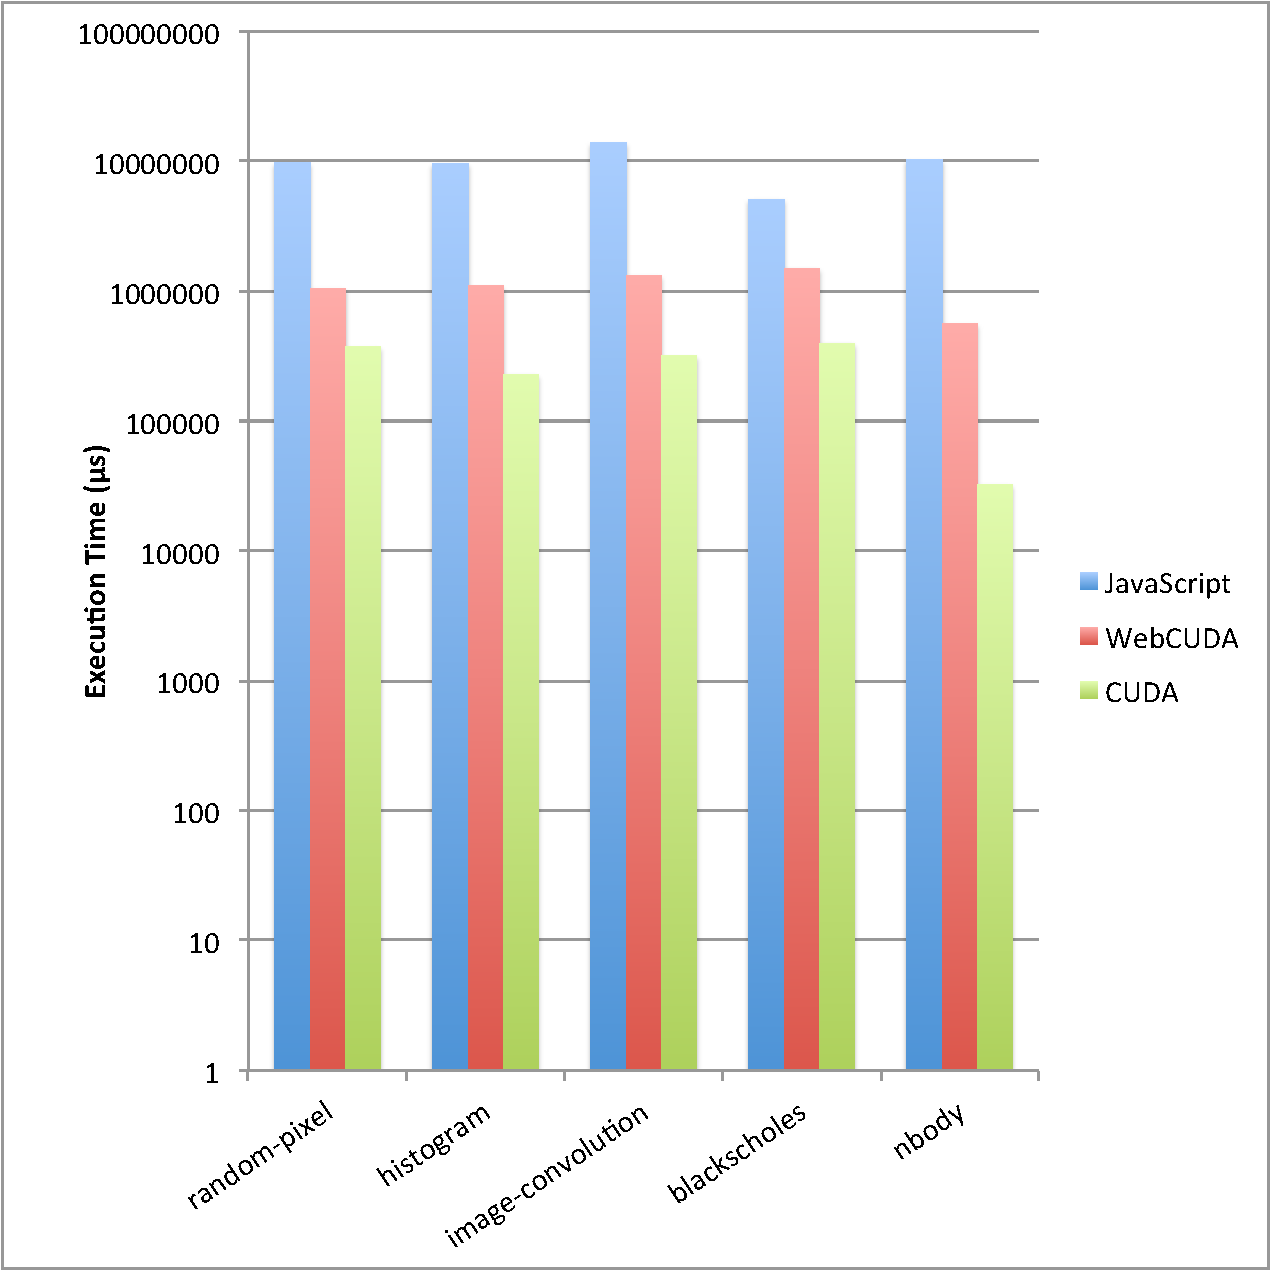
\includegraphics[width=\columnwidth]{./figures/fig1}
	\end{center}
	\caption{Creating new \name Device Object}
	\label{v8codea}
\end{figure}

\begin{figure}
	\begin{center}
		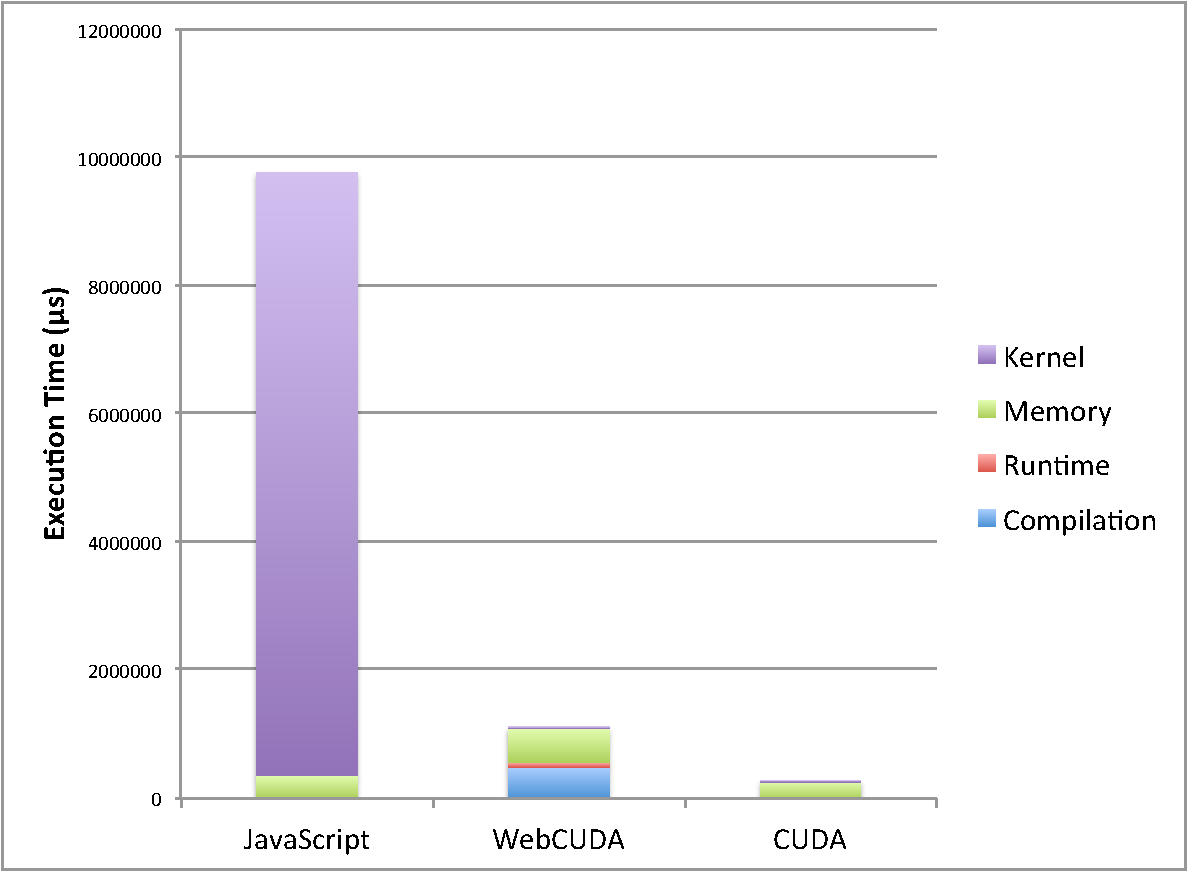
\includegraphics[width=\columnwidth]{./figures/fig2}
	\end{center}
	\caption{Creating new \name Device Object}
	\label{v8codea}
\end{figure}

\subsection{Benchmarks}
there should probably be a table here...
%TODO make table listing benchmarks, data sets
\begin{table}
	\begin{center}
		\begin{tabular}{| l | l |}
			\hline
			Benchname & Input Size \\
			\hline
			random-pixel & N/A \\
			\hline
			Nbody &  1024 bodies \\
			\hline
		\end{tabular}
	\end{center}
	\caption{Description of Benchmarks use for evaluation.}
	\label{benchmark-table}
\end{table}

\paragraph{Random Pixel Generator}

\paragraph{N-Body Force Calculation}

\paragraph{Black Scholes} \hspace{0pt}\\
I am curious what this does


\paragraph{Histogram}
maybe want it this way instead \ldots

\paragraph{Awesome B}

\subsection{Experimental Setup}

\subsection{Results}

\paragraph{Execution Time}
\paragraph{Compilation Overhead}
\paragraph{CUDA Visual Profiling}
\paragraph{V8 Runtime Overhead}
something about how the overhead is infinitesimal and does not influence
decisions about whether to run a program on the GPU or not
\paragraph{Running Native JavaScript Programs}




\section{Discussion}
\label{disc}

\subsection{Challenges Encountered}
While our idea of adding CUDA bindings to JavaScript and the final
implementation is straightforward, there was much experimentation to get to this point.
One of the main obstacles encountered during this project is understanding the
V8 code base. The non-machine backend specific section of code is around 200K
LOC. In addition, there is not a definitive source explaining the compiler: some
blogs exist, but they oftentimes cover good programming practices for code to
performs well on the v8 compiler as opposed to explaining how the compiler works
itself. Therefore, it is necessary to look at the code itself to determine the
best way to interact with the compiler.

Luckily, two of the authors of the paper have had much experience working with
the v8 codebased and thus did not have such a steep learning curve. However, v8
is a ongoing project and is rapidly changing. Because of this, we wanted to work
on the most recent version to give our project the most relevance. The author's
previous experience was on a version of v8 from 2012. While the basic structure
of the compiler in both versions was similar, the authors were astonished to
find how many of the class and method names had changed. There was a major
overhaul of the external programmers API last summer, which has made most
information provided is blogs obsolete. Even Google's Embedder's Guide
Documentation \cite{embeddersGuide} does not correspond to the updated API.
Therefore, it took longer than expected to implement \name and caused many
headaches. Thankfully, with our newfound experience with this version of v8, any
additional changes necessary to be made to \name should be straightforward to
implement.

\subsection{WebCUDA Limitations}
While the current \name specification and implementation has enough
functionality for many CUDA implementations, many CUDA Runtime features do not
have a mapping in \namens. Below we highlight some limitations of \namens.

\subparagraph{Streaming Memory}
 One of the major limitations of \namens, as seen in
Section~\ref{eval}, is the lack of support for CUDA Streaming Memory
\cite{cuStream}. The authors felt Streaming Memory is not a core
CUDA feature and felt is was outside of the scope of this project.
Luckily, there is no fundamental reason CUDA Streams cannot be integrated into 
\name and can easily be added in future versions.

\subparagraph{Multiple Dimensioned Arrays}
As JavaScript implements multiple dimensioned arrays, as an array of potentially
non-contiguous arrays, it is not clear how to extend \name to include
support for multiple dimension array memory transfers between the host and
CUDA-enabled device. While this affects the ease of programmability, it does not
limit the range of programs which can be ported to \namens.

\subparagraph{Programmability} Many libraries, such as thrust~\cite{thrust} and
many math libraries~\cite{magma, cuSparse, arrayFire}, exist to simplify CUDA
programming. Unfortunately, these libraries are unavailable in the \name environment. While
this is a current setback, as CUDA programming in the browser becomes prevalent,
inevitably tools will be created to simplify the process GPGPU programming in
this domain.

In addition, the CUDA runtime is able to perform many actions necessary to
connect to a CUDA device without the programmers knowledge that the programmer
must explicitly perform in \namens, such as creating a CUDA context and
connecting to a device. \name can be extended to perform many of the same
monitoring features as the CUDA Runtime, but this would require a nontrivial
amount of effort to implement. The authors decided to leave this as future work,
as this does not limit the capabilities of \namens.

\subparagraph{Performance}
asynchronous calls


\subparagraph{The Great Unknown}

\subsection{Programmability}
want something here about how easy it is to write webcuda programs. (change section title accordingly)

\subsection{Security}
\subsection{Future Work}


\section{Related Work}
\label{related}

\paragraph{WebCL}
something

\paragraph{ParallelJS}
Talk about this paper \cite{parallelJS} something about it

\paragraph{JCuda, Python Cuda}


\section{Conclusions}


\appendix
\section{Appendix Title}

This is the text of the appendix, if you need one.

\acks

Acknowledgments, if needed.

% We recommend abbrvnat bibliography style.

\bibliographystyle{abbrvnat}

% The bibliography should be embedded for final submission.

\begin{thebibliography}{}
\softraggedright


\bibitem[Wang et~al.(2014)Wang, Jin]{paralleljs}
J. Wang, N. Rubin, and S. Yalamanchili. \newblock ParallelJS: An Execution Framework for JavaScript on Heterogeneous Systems
\newblock In \emph{GPGPU-7}, March 2014.

\bibitem[Aang et~al.(2014)Aang, Jin]{doxygen}
Doxygen



\end{thebibliography}


\end{document}

%                       Revision History
%                       -------- -------
%  Date         Person  Ver.    Change
%  ----         ------  ----    ------

%  2013.06.29   TU      0.1--4  comments on permission/copyright notices

